\section{Stanowiska badawcze}
W~niniejszym rozdziale opisane zostaną stanowiska przygotowane do przeprowadzenia kolejnych badań.

\subsection{Niezależne podstawowe stanowiska}
Pierwszym etapem prac mających na~celu przygotowanie stanowisk badawczych było skonfigurowanie podstawowej wersji obu stanowisk wraz ze wszystkimi dostępnymi elementami. Stanowiska zostały skonfigurowane i~uruchomione w sposób całkowicie nie zależny od siebie.

Konfigurację obu sterowników wraz z modułami przedstawiają Rysunki~\ref{conf:cp}~oraz~\ref{conf:cx}. Tak stworzone konfiguracje pozwoliły uzyskać odpowiednio topologię jak na Rysunku~\ref{topology:cp} dla stanowiska typu CP oraz jak na Rysunku~\ref{topology:cx} dla stanowiska typu CX.
\begin{figure}[!htb] 	\centering 	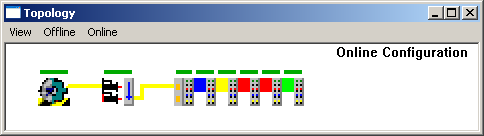
\includegraphics[width=0.9\textwidth]{images/topologyCP} \caption{Topologia stanowiska typu CP} \label{topology:cp} \end{figure}
\begin{figure}[!htb] 	\centering 	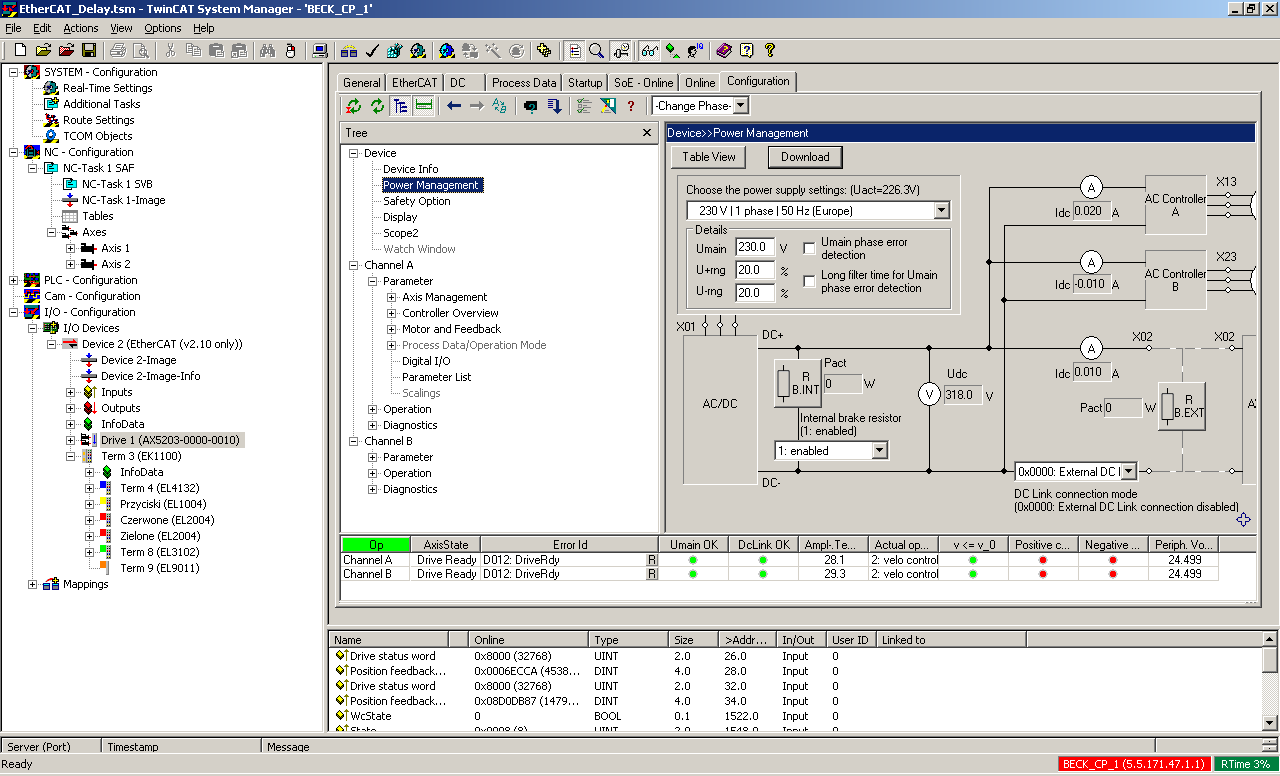
\includegraphics[width=0.99\textwidth]{images/confCP} \caption{Konfiguracja stanowiska typu CP} \label{conf:cp} \end{figure}

\begin{figure}[!htb] 	\centering 	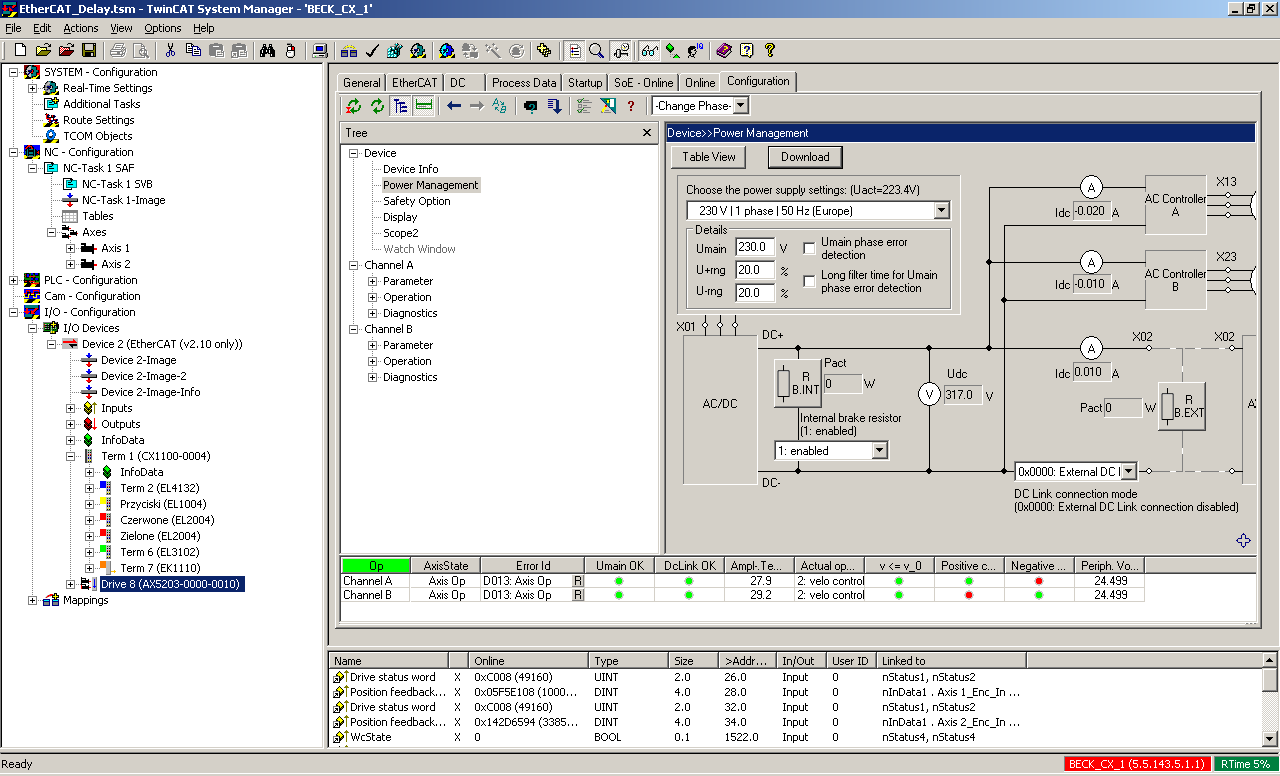
\includegraphics[width=0.99\textwidth]{images/confCX} \caption{Konfiguracja stanowiska typu CX} \label{conf:cx} \end{figure}
\begin{figure}[!htb] 	\centering 	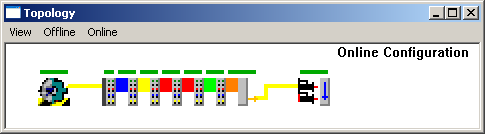
\includegraphics[width=0.9\textwidth]{images/topologyCX} \caption{Topologia stanowiska typu CX} \label{topology:cx} \end{figure}

Głównym problemem związanym z~uruchomieniem pełnych możliwości stanowisk było prawidłowe skonfigurowanie oraz uruchomienie serwomechanizmów napędzanych przez moduł~AX5203.
%\subsection{Opóźnienia pojedynczego odcinka sieci}
%\subsection{Wpływ topologi na opóźnienia}
%\subsection{Czas stabilizacji sieci po zmianach}
%
%Różne kable
%Długość kabla
%

%Połączyć do jednego sterownika oba napędy kolejno i zrobić coś na zasadzie inkrementacji i sprawdzić czy się przypadkiem nie rozjedzie
%
%Mamy opóźnienie na jednym odcinku
%
%Ewentualnie jeden kabel można zamienić na dłuższy i sprawdzić czy nie ma różnicy.
%
%Wymyślić jak sprawdzić czas ponownego włączenia do sieci.